\documentclass[10pt]{article}
\usepackage[margin=0.85in]{geometry}
\usepackage{amsmath,amssymb,graphicx,booktabs,longtable,hyperref}
\title{Finite-Sample Support-Size Testing: Certified Decisions, Sequential Costs, and Failure Modes}
\author{Anonymous research draft}
\date{}
\begin{document}\maketitle
\section*{Abstract}
Support-size testing distinguishes distributions supported on at most n categories from distributions whose probability mass outside the n most likely categories is at least epsilon. Asymptotically optimal testers do not by themselves determine useful finite-sample constants or acquisition costs. We study certified Chebyshev statistics combined with independent acceptance validation and a count-test fallback. Across 69,896,000 method-trial evaluations, we compare tuned single-scale and multiscale families, FH-shaped practical variants, literal finite-scale reference branches, and stronger count baselines. On the labelled-stream grid, the multiscale hybrid uses 68.83\% of the immediate count baseline's samples on Yes instances and 85.11\% on No instances, with validation included. Large-scale checkpoint results show larger apparent gains, demonstrating why stopping-rule fairness matters. We also measure effective-support lower-bound power, independently retest searched difficult distributions, and expose sensitivity to natural group dependence. The hybrid has a finite-sample error guarantee under iid sampling, but we do not claim a new optimal-order sample-complexity theorem or universal empirical dominance.

\section*{1. Introduction}
Counting observed categories is reliable as a lower bound but can require many observations when mass is dispersed among rare categories. Polynomial extrapolation can infer support beyond the observed count. The difficulty is that approximation error, sampling fluctuation, repeated looks, and data dependence all interact. A small-budget statistic that frequently rejects alternatives can still be unusable because it rejects null distributions too often.

The supplied manuscript Optimal Support Size Testing establishes an asymptotically optimal tester and a stronger effective-support lower bound [1]. Our aim is to make the finite-sample experimental questions explicit. We investigate which component creates savings, whether those savings survive a competitive stopping rule, which distributions defeat the chosen practical constants, and what changes when records share documents, users, orders, or sampling events.

Our contribution is a reproducible finite-sample study and certified implementation, rather than a replacement of the original optimality proof. The artifact includes interval-certified thresholds, exact integer rejection decisions, a corrected sequential ablation, a fair labelled-stream benchmark, held-out adversarial testing, and raw outcomes supporting all reported tables. These components expose both useful operating regimes and important limits.

\section*{2. Problem and related work}
\[
H_0:S=|\operatorname{supp}(p)|\le n,\qquad H_1:\Delta_n(p)=\sum_{i>n}p_{(i)}\ge\varepsilon.
\]
The probabilities p\_(i) are ordered decreasingly. Instances with S>n and Delta\_n<epsilon are a promise gap; neither binary output is scored as an error there. A non-rejection from a fixed-budget one-sided polynomial test is reported as Inconclusive, not as a certified Yes. A sequential hybrid returns a binary result only after a certified acceptance or the final count budget.

The original Wang construction uses multiple Chebyshev scales and attains order n/(epsilon log n) [1]. Ferreira Pinto Jr. and Harms study the same promise problem using a single polynomial with an additional logarithmic dependence on epsilon [2]. We distinguish their literal conservative finite-scale branch from a tuned FH-shaped statistic, and from a separately certified FH-shaped variant. This distinction is necessary because changing constants or thresholds does not preserve the cited theorem automatically.

Wu and Yang study support estimation under a minimum nonzero mass assumption [3]. Regularized weighted Chebyshev estimators also target support estimation with additional model structure [4]. Those are valuable related methods, but an oracle lower bound on minimum mass would change our distribution-free promise problem. We therefore do not present a tuned point estimator as a universally valid tester. Chao1 thresholding is included only as a clearly labelled heuristic diagnostic. Time-uniform inference motivates careful error spending [5]; the present construction uses a finite, predetermined look schedule rather than an unrestricted confidence sequence.

\section*{3. Certified finite-sample construction}
Under Poissonized sampling with predetermined mean m, category counts N\_i are independent Poisson(m p\_i). At a scale with A=ma and B=mb, define Chebyshev weights f(0)=0 and f(l)=1 for l above degree k, using the original polynomial recurrence for the remaining coefficients. The statistic is Z=sum\_i f(N\_i)=D+sum\_{l=1}^k F\_l(f(l)-1). Parameters are fixed before evaluating a test sample.

\[
\rho=\frac1{T_k((B+A)/(B-A))},\quad R=\max\{0,1,f(1),\ldots,f(k)\}-\min\{0,1,f(1),\ldots,f(k)\}.
\]
Every proposed scale is checked using Arb interval arithmetic: 0<A<B<=m, k<=sqrt(B(B-A)), and the configured weight cap. Degree is reduced or the scale is omitted if certification fails. Under these premises, the polynomial expectation envelope gives E[Z]<=(1+rho)S. A single-scale comparator spends its error budget on its one predetermined scale, rather than inheriting the multiscale penalty.

\[
u=R\sqrt{\frac n2\log\frac{HK}{\delta}},\qquad Z>(1+\rho)n+u\ \Longrightarrow\ \mathrm{No}.
\]
Arb supplies upper bounds for rho, the range, and thresholds, and lower bounds for statistic coefficients. All final rejection comparisons use a common binary-rational denominator and integers. Floating calculations only identify candidates for this exact comparison. This protects the analytical null guarantee from rounding-induced false rejection. The random samplers themselves use standard double-precision numerical libraries; they are not formally verified random-number implementations.

The multiscale family proposes a\_j=2^j epsilon/(8n), with B proportional to log(en). The single-scale family selects one j independently on development data. The practical FH-shaped family proposes a proportional to epsilon log(1/epsilon)/n, b proportional to epsilon log(en)^2/[n log(1/epsilon)], and degree proportional to log(en). Its certified version is checked by the same envelope and concentration argument. Its native-threshold version uses the FH-shaped raw statistic with threshold (1+epsilon/2)n and has no inherited finite-sample guarantee after tuning.

\section*{4. Sequential decisions and guarantees}
Training batches are independent Poisson increments on predetermined increasing means. Directly observing the (n+1)-st category permits immediate rejection. Polynomial rejection is checked only at the fixed looks. To accept early, the algorithm freezes the observed training set A, draws r fresh independent validation labels, and counts V labels outside A. The singleton heuristic F1/m gates whether to spend validation labels; it never certifies acceptance.

\[
\Pr\{\operatorname{Bin}(r,\varepsilon)\le k\}\le\frac\delta{2H},\quad V\le k\ \Longrightarrow\ \mathrm{Yes}.
\]
The final count budget m* is the smallest proposed integer certified to satisfy Pr(Poisson(m* epsilon)<=n)<=delta/2 when validation is enabled. Without early acceptance, the full delta is assigned to the count fallback. Total scheduled validation labels are capped at m*/5. This correction prevents the polynomial-only ablation from wasting half its false-negative budget on a branch it does not use.

Proposition 1 (conditional on the iid model). With fixed n, epsilon, delta, fixed configuration, independent sampling randomization, fresh validation samples, and the certified comparisons above, the probability of a No output under S<=n is at most delta, and the probability of a Yes output under Delta\_n>=epsilon is at most delta. The worst expected acquisition cost is O((n+log(1/delta))/epsilon). No minimum positive category probability is assumed.

Proof. Under S<=n, append zero contributions to obtain n independent bounded terms. Hoeffding bounds each polynomial crossing by delta/(HK); the union bound covers all scales and looks even though looks share observations. A direct count rejection is impossible under the null. Under the alternative, any history-dependent set A with at most n elements has outside mass at least epsilon. Conditional on that history, fresh validation gives a binomial lower-tail error at most delta/(2H). Before discovery of the (n+1)-st category, the probability of a new category is at least epsilon. Coupling discoveries with Bernoulli(epsilon) trials yields the fixed-size bound Pr(D<=n)<=Pr(Bin(M,epsilon)<=n), and Poisson mixing yields the certified final tail bound. An error on a path reaching fallback is a subset of the error event for the full potential training path. Summing validation and fallback errors gives delta. Training means and all scheduled validation sizes bound expected acquisition by 1.2m*. Standard Poisson concentration gives the stated order. Immediate direct-count stopping only shortens a path and adds no null errors.

\section*{5. Experimental design}
The main grid uses n in {1,000,10,000,100,000,1,000,000}, epsilon in {0.001,0.005,0.01,0.02,0.05,0.1,0.2}, eleven distribution scenarios, thirteen budget factors C from 0.5 through 16, and an additional certified count budget. Each method cell has 2,000 trials, split across four independently keyed random blocks. Equal-probability category groups permit exact occupancy-profile simulation without enumerating up to 100 million categories. The sampler preserves groups of distinct categories; it does not replace a rare tail by one category.

Each of the multiscale, single-scale and FH-shaped families received eight development candidates. Development uses n=1,500 and 15,000, epsilon=0.005,0.05,0.2, different distribution shape parameters, four budgets, and 400 trials per cell. Certified candidates are ranked by mean non-rejection on alternatives; the native heuristic additionally receives a penalty for observed null inflation. No formal outcomes alter the selected configurations. The selected multiscale B factor is 1.000, weight cap 10.000, and the selected single scale is j=4.

A local prospective design and code/data hashes were recorded before formal evaluation. A subsequent correctness audit found nominal equality-boundary distributions infinitesimally below epsilon after exact rational normalization. The original outputs remain in a superseded archive. We repaired the constructor, retained the original selected configurations, recorded the amendment, and reran every formal suite with the same keyed seeds. Exact normalized tail certificates are provided. This transparent amendment is not an external preregistration claim.

\begin{table}[htbp]\centering\small\caption{Experimental inventory. Method-trial evaluations reuse common samples across methods; they are not independent datasets.}
\resizebox{\linewidth}{!}{
\begin{tabular}{lll}
\toprule
Suite & Method cells & Method-trial evaluations \\
\midrule
fixed & 25,872 & 51,744,000 \\
sequential & 792 & 1,584,000 \\
adversarial\_fixed & 1,080 & 10,800,000 \\
adversarial\_sequential & 216 & 1,080,000 \\
stream & 240 & 240,000 \\
structure & 432 & 432,000 \\
group\_holdout & 432 & 864,000 \\
sensitivity & 696 & 3,120,000 \\
reference & 32 & 32,000 \\
\bottomrule
\end{tabular}
}
\end{table}
Error rates use one-sided exact Clopper-Pearson bounds. We report 95\% simultaneous bounds with Bonferroni correction across all non-Gap method cells in each frozen suite. The three lower-bound failure metrics form a separate simultaneous family in the fixed-budget suite. The smallest passing budget m* is defined by simultaneous upper bounds across all promised scenarios, not by an observed error-rate threshold. No passing tested budget is reported as right censoring.

Cost contrasts use common training paths and independent shared validation pools. Cell means are weighted equally, with Yes and No strata separate. Paired Monte Carlo intervals use delta-method standard errors; Holm correction applies to the reported aggregate cost contrasts. A separate scenario bootstrap describes sensitivity to the finite grid composition, not generalization to arbitrary unknown distributions. The full seed-block table and trial arrays are released.

\section*{6. Fixed-budget risk, scaling, and scale contribution}
Across the fixed-budget grid, the largest observed null rejection rate among the three certified polynomial families is 0.05\%. Complete-grid passing budgets were found for Chao1 point threshold: 0/28 parameter pairs, Observed count: 28/28 parameter pairs, Certified FH-shaped: 28/28 parameter pairs, FH-shaped native threshold: 15/28 parameter pairs, Certified multiscale: 28/28 parameter pairs, Tuned single scale: 28/28 parameter pairs. Native-threshold or point-estimate performance must be assessed jointly on nulls and alternatives; high rejection power alone is not evidence of a valid test.

\begin{figure}[htbp]\centering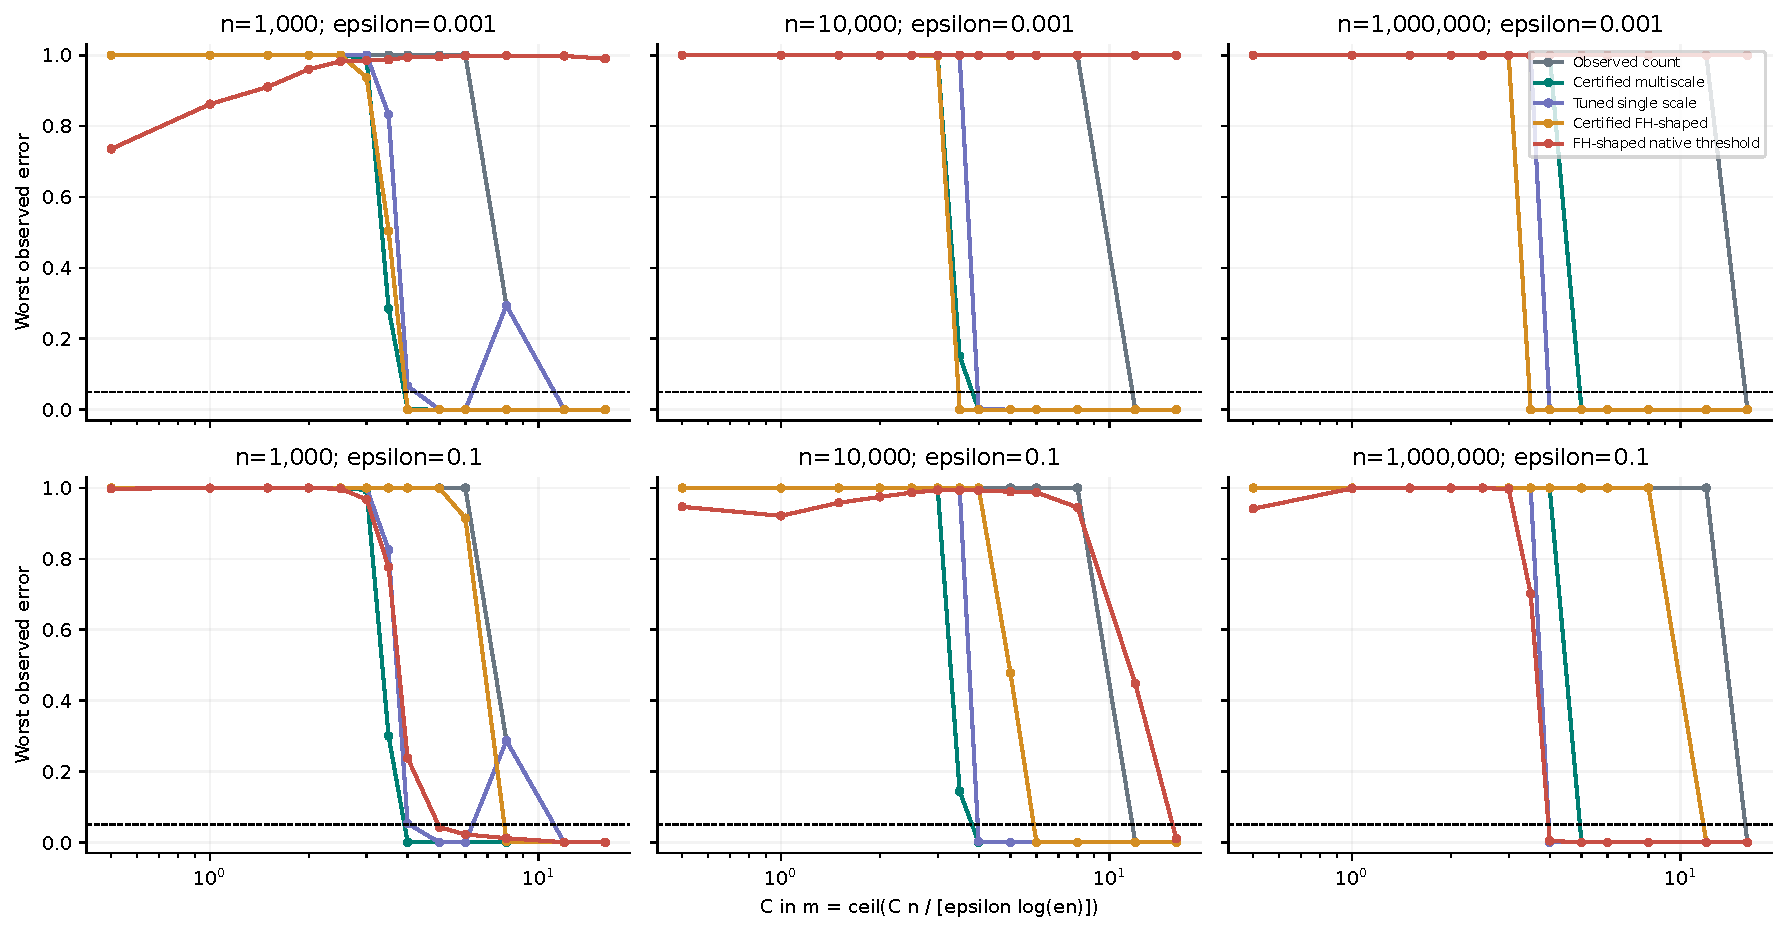
\includegraphics[width=\linewidth]{figures/fixed_risk.pdf}\caption{Worst observed error over promised synthetic scenarios. The dashed line is 5\%; simultaneous confidence bounds, not this point-estimate plot, determine passing budgets.}\end{figure}
\begin{figure}[htbp]\centering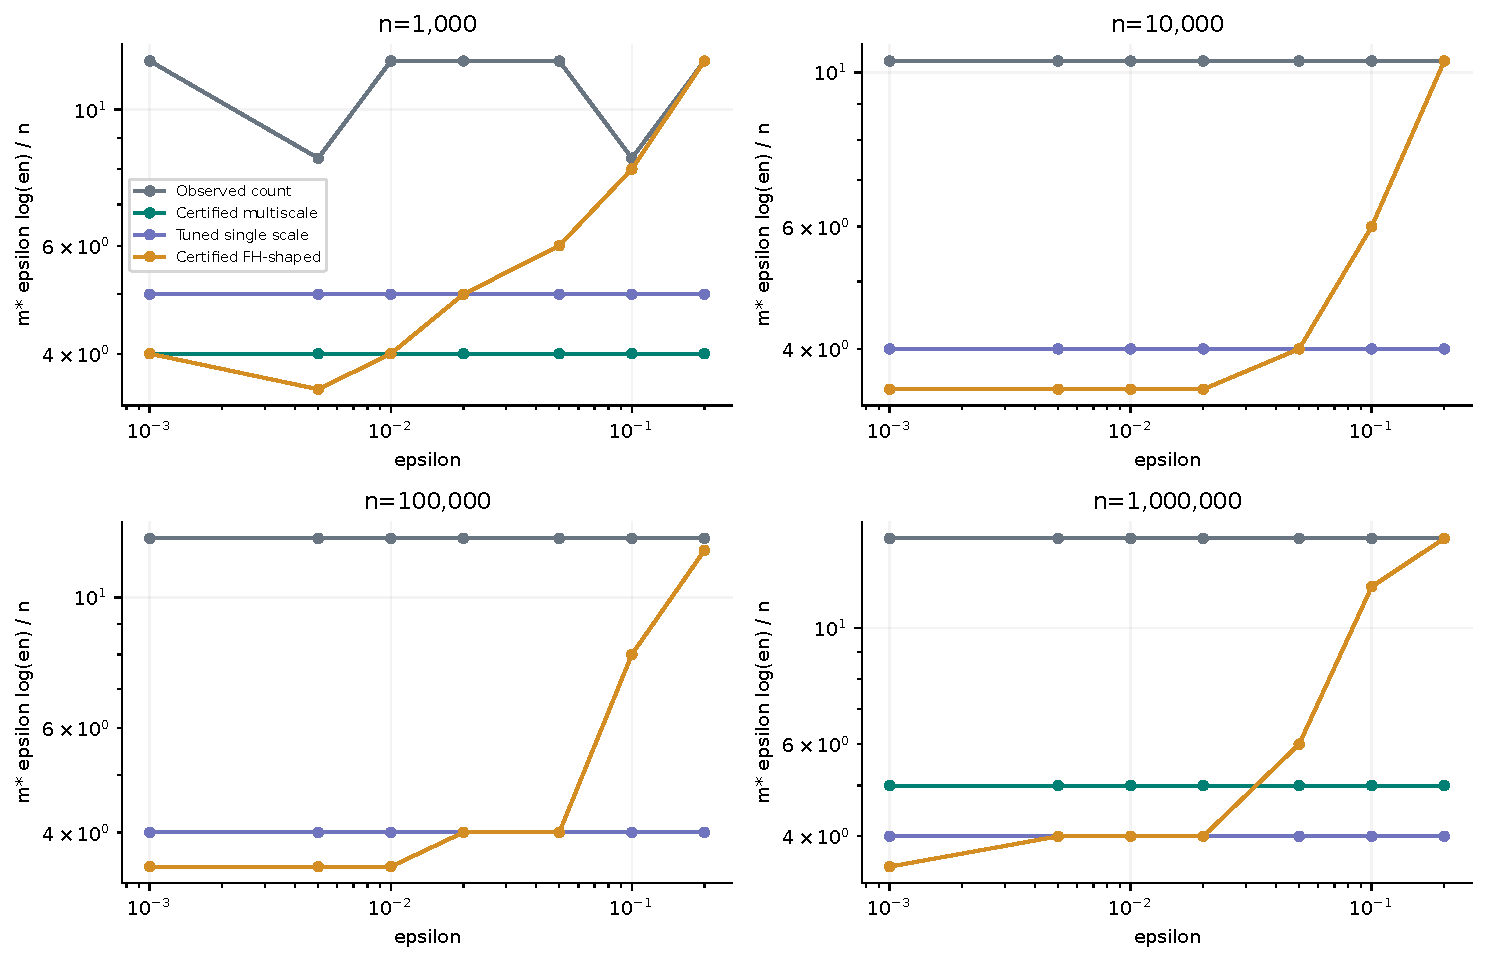
\includegraphics[width=\linewidth]{figures/sample_complexity.pdf}\caption{Smallest tested budget passing simultaneous 95\% error upper bounds across all promised synthetic scenarios. Missing points are right-censored; no interpolation or universal complexity claim is made.}\end{figure}
The normalized sample-complexity curves assess finite-grid scaling as epsilon decreases. They do not prove that practical constants retain the original optimal order. In particular, both the finite concentration correction and the fallback may dominate difficult small-n regimes. A missing point is a failure to establish the target error level with this grid and Monte Carlo precision, not proof that no possible budget works.

\begin{table}[htbp]\centering\small\caption{Comparator budgets relative to multiscale m* across 28 n/epsilon pairs. Smaller means the comparator outperforms multiscale on this finite-grid criterion.}
\resizebox{\linewidth}{!}{
\begin{tabular}{llll}
\toprule
Comparator & Smaller budget & Equal budget & Larger budget \\
\midrule
Tuned single scale & 7 & 14 & 7 \\
Certified FH-shaped & 12 & 5 & 11 \\
Observed count & 0 & 0 & 28 \\
\bottomrule
\end{tabular}
}
\end{table}
The comparison does not show uniform multiscale superiority. At n=1,000, the multiscale family passes at approximately C=4 whereas the tuned single-scale family needs C=5; at n=1,000,000 the ordering reverses, with single scale passing at C=4 and multiscale at C=5. Certified FH-shaped variants also beat multiscale on several small-epsilon settings. Consequently, these experiments do not empirically establish the asymptotic logarithmic-factor advantage of the original theorem for the practical implementations. The finite-sample evidence supports regime-dependent method selection and careful certification, rather than a blanket best-method claim.

\begin{figure}[htbp]\centering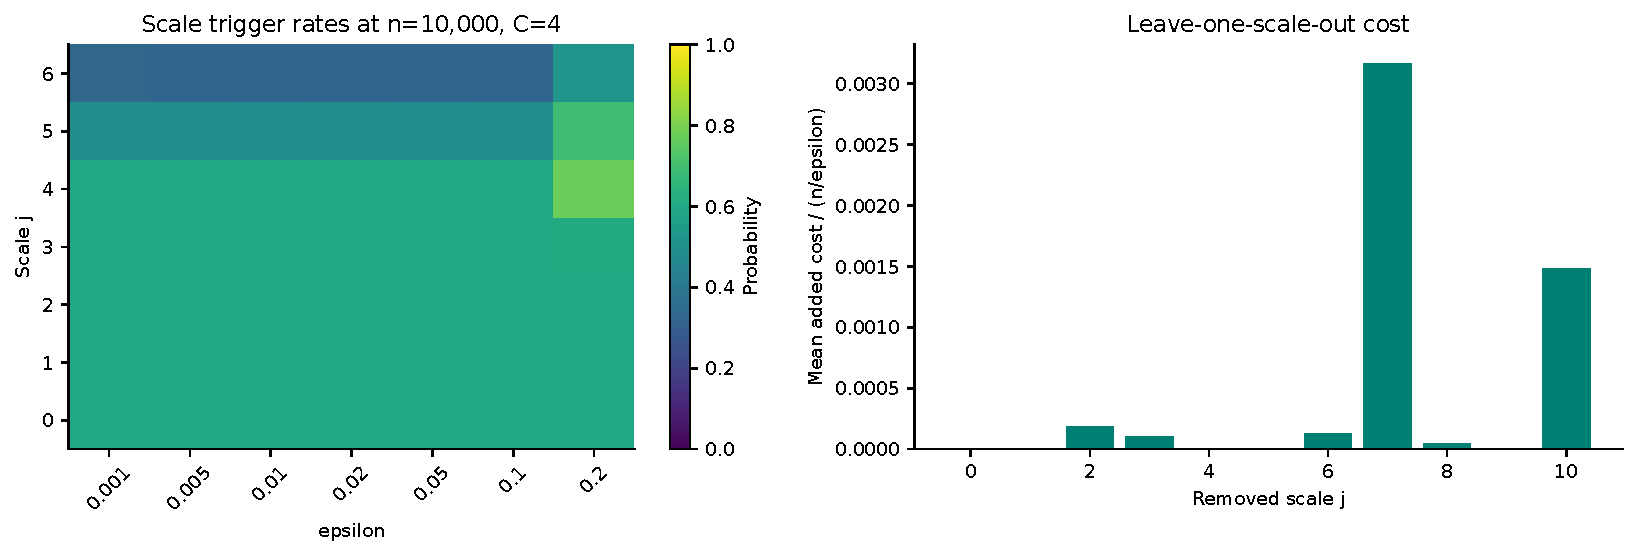
\includegraphics[width=\linewidth]{figures/scale_mechanism.pdf}\caption{Left: all triggered scales are recorded, not only the first winner. Right: remove one scale while retaining the original error spending and common sample paths.}\end{figure}
Scale diagnostics record all crossings, exclusive crossings, first winning scale, and additional sequential cost when a single scale is removed. The removal experiment retains the original thresholds, isolating the information contributed by that scale; it is not a newly optimized smaller family. The independent single-scale development search prevents a weak fixed j=0 comparator from mechanically favoring multiscale testing.

\section*{7. Sequential efficiency and actual acquisition cost}
\begin{table}[htbp]\centering\small\caption{Equal-weight mean cost ratios. Large-scale trajectories use checkpoint count as denominator; labelled streams use immediate fixed count.}
\resizebox{\linewidth}{!}{
\begin{tabular}{llll}
\toprule
Suite & Method & Yes ratio & No ratio \\
\midrule
sequential & Count + validation & 0.265 & 1.002 \\
sequential & Polynomial + count & 1.000 & 0.560 \\
sequential & Single-scale hybrid & 0.265 & 0.569 \\
sequential & FH-shaped hybrid & 0.265 & 0.619 \\
sequential & Multiscale hybrid & 0.265 & 0.560 \\
stream & Checkpoint count & 1.003 & 1.432 \\
stream & Count + validation & 0.688 & 1.002 \\
stream & Polynomial + count & 1.003 & 0.849 \\
stream & Single-scale hybrid & 0.688 & 0.894 \\
stream & FH-shaped hybrid & 0.688 & 0.895 \\
stream & Multiscale hybrid & 0.688 & 0.851 \\
\bottomrule
\end{tabular}
}
\end{table}
On the large-scale sequential grid, the full hybrid uses 26.47\% and 55.98\% of checkpoint-count cost in Yes and No cases, respectively. Its maximum observed false-positive rate is 0.00\%, and its maximum observed false-negative rate is 0.10\%. These are finite-grid observations alongside, not replacements for, the analytical guarantee.

\begin{figure}[htbp]\centering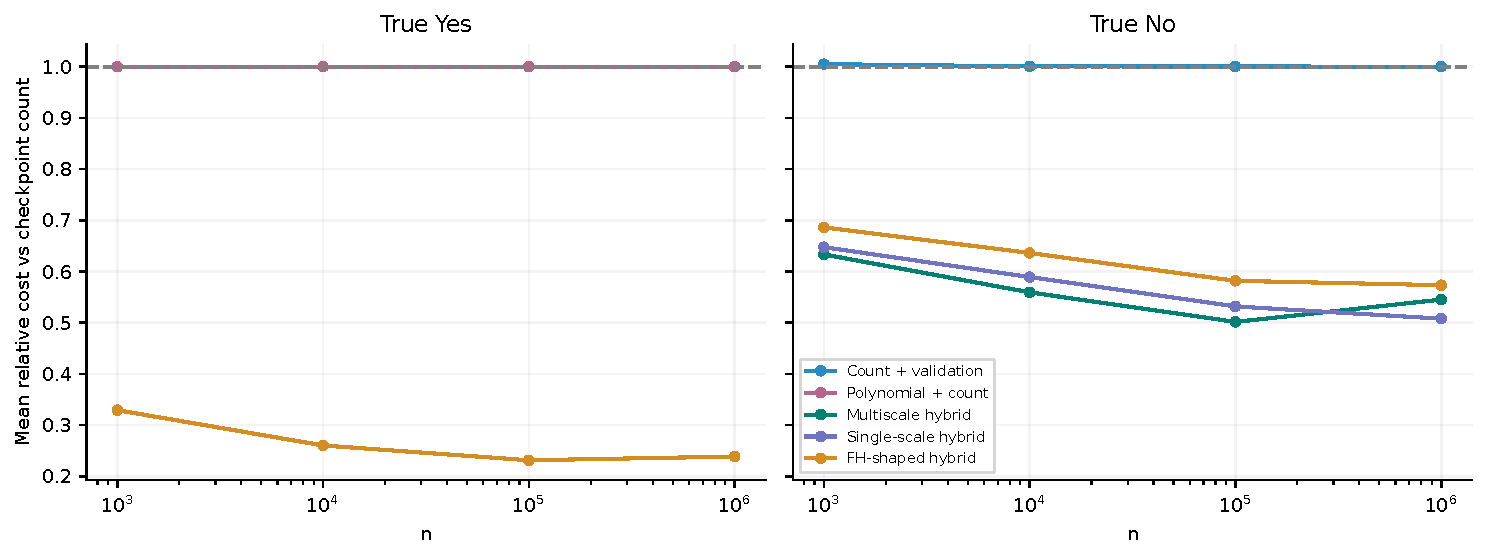
\includegraphics[width=\linewidth]{figures/sequential_ablation.pdf}\caption{Large-scale coupled Poisson trajectories. Cost is stopped training mean plus validation labels; it estimates expected acquisition cost and is not the distribution of actual sample counts.}\end{figure}
In the actual labelled-stream suite, n ranges from 50 to 1,000, epsilon is 0.01 or 0.1, and each cell has 1,000 trials. The hybrid reduces mean cost by 31.17\% on Yes cases and 14.89\% on No cases compared with immediate fixed count. The worst relative costs in those strata are 1.051 and 1.000. A method may therefore lose on individual configurations even when its equal-weight mean improves.

\begin{figure}[htbp]\centering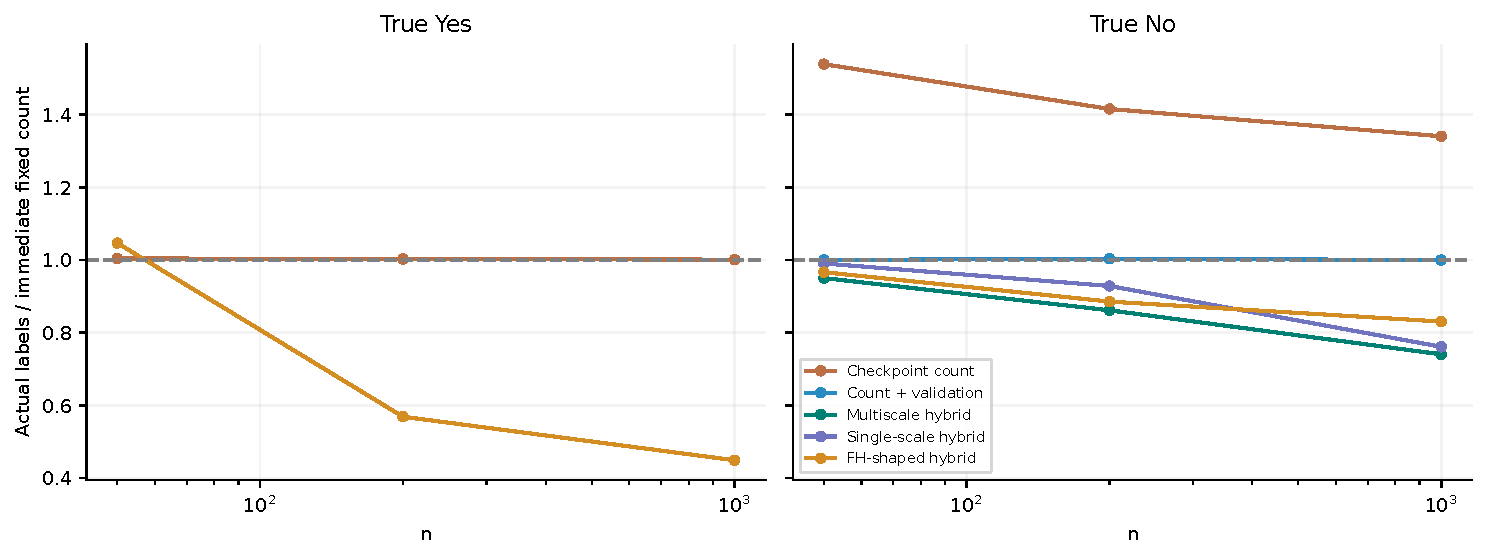
\includegraphics[width=\linewidth]{figures/actual_cost.pdf}\caption{Actual label consumption including validation, compared with an immediately stopping fixed-budget count baseline. All methods share iid training labels and fresh validation pools.}\end{figure}
\begin{figure}[htbp]\centering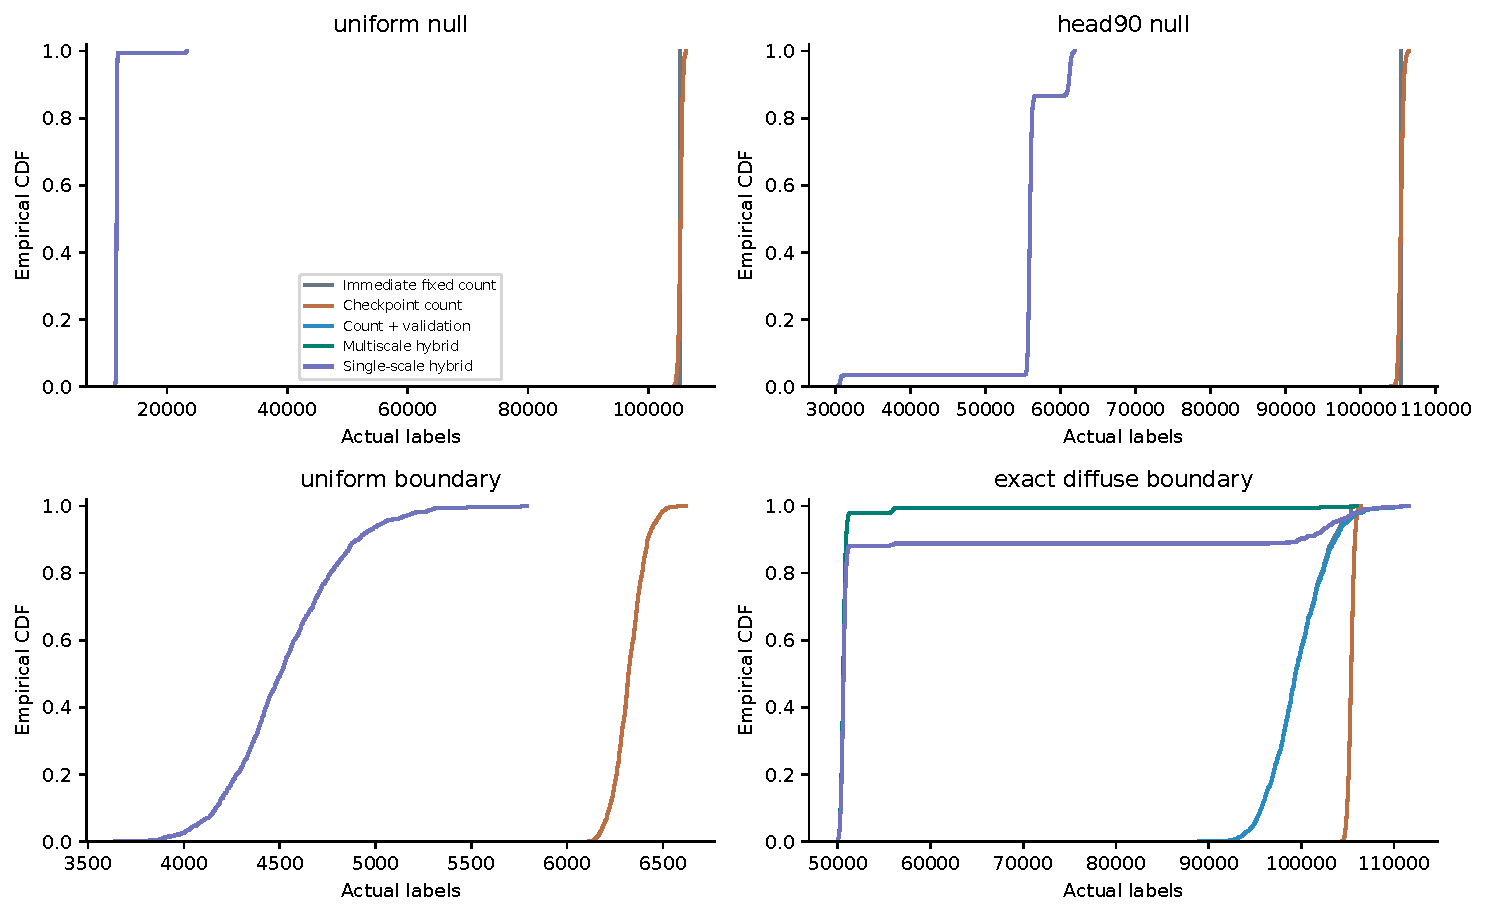
\includegraphics[width=\linewidth]{figures/actual_cost_cdf.pdf}\caption{Full stopping-cost distributions for n=1,000 and epsilon=0.01. Quantiles refer to actual consumed labels, with verification samples included.}\end{figure}
\begin{table}[htbp]\centering\small\caption{Paired actual-cost contrasts: multiscale hybrid minus comparator, normalized by immediate fixed-count mean. Negative values favor the hybrid. Intervals describe Monte Carlo uncertainty on this fixed grid.}
\resizebox{\linewidth}{!}{
\begin{tabular}{lllll}
\toprule
Truth & Comparator & Difference & 95\% MC interval & Holm p \\
\midrule
No & Immediate fixed count & -0.149 & [-0.150, -0.148] & <1e-300 \\
No & Count + validation & -0.151 & [-0.151, -0.150] & <1e-300 \\
No & FH-shaped hybrid & -0.043 & [-0.044, -0.042] & <1e-300 \\
No & Single-scale hybrid & -0.043 & [-0.044, -0.041] & <1e-300 \\
Yes & Immediate fixed count & -0.312 & [-0.314, -0.310] & <1e-300 \\
Yes & Count + validation & 0.000 & [0.000, 0.000] & 1 \\
Yes & FH-shaped hybrid & 0.000 & [0.000, 0.000] & 1 \\
Yes & Single-scale hybrid & 0.000 & [0.000, 0.000] & 1 \\
\bottomrule
\end{tabular}
}
\end{table}
The count baseline stops at the exact observation that first reveals category n+1 and otherwise stops at its interval-certified fixed budget. All hybrids also permit immediate direct-count rejection; validation labels are fully charged. This study separates a genuine improvement in inference from savings caused by an artificially delayed baseline. Poisson stopped-mean quantiles from compressed simulations are never presented as actual acquisition quantiles.

\section*{8. Adversarial and effective-support evaluation}
The search enumerates head-tail and multi-level shapes with tail-size factors 2,10,100,1,000, tail exponents, boundary ratios, and lognormal nulls. For each of six n/epsilon pairs, three nulls and three alternatives are selected by fixed-budget error and then sequential cost. All 36 selected distributions are frozen before independent tests with 10,000 trials per fixed-budget cell and 5,000 per sequential cell. Candidate scores, selected probabilities, exact promise checks and raw retest outcomes are retained.

For the multiscale fixed test, the largest independently observed alternative non-rejection rate at C=4 is 0.02\%. This directly tests whether ordinary benchmark success persists near searched difficult cases. Search is restricted to the stated families; it is not a proof of a least favorable distribution over the full simplex.

\begin{figure}[htbp]\centering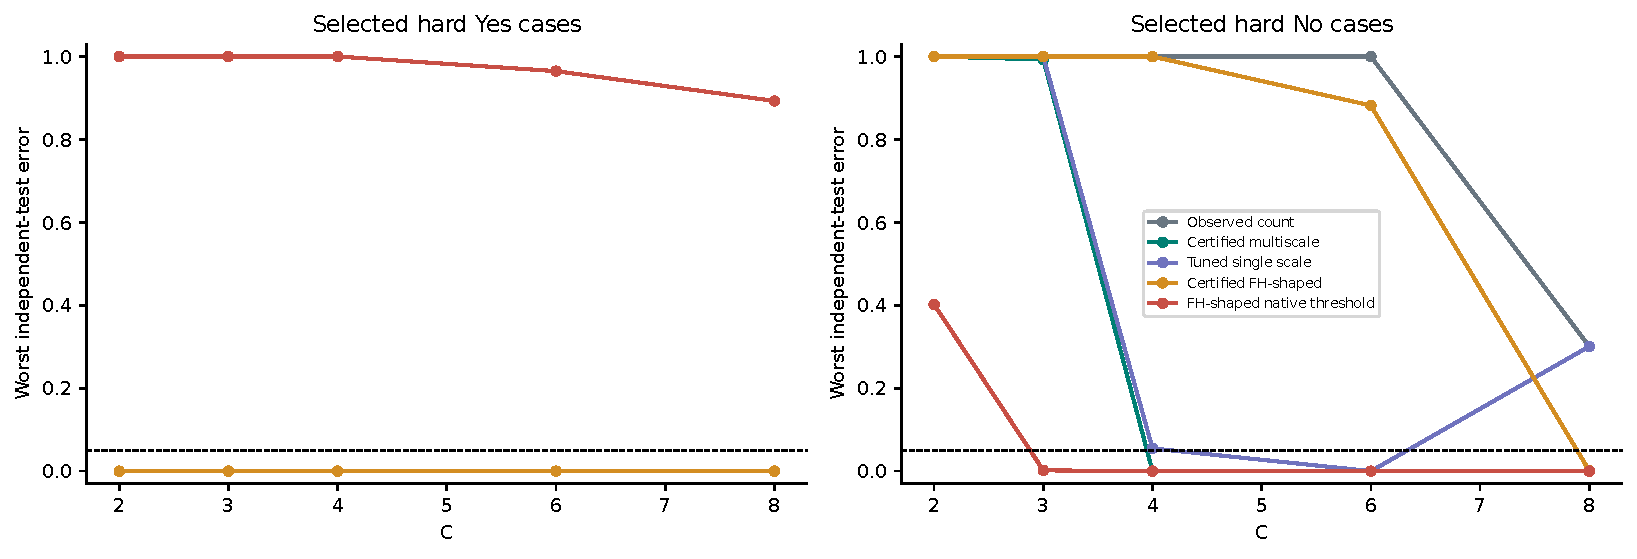
\includegraphics[width=\linewidth]{figures/adversarial_risk.pdf}\caption{Adversarial candidates were selected on a separate search stream and then frozen. Each fixed-budget test cell uses 10,000 new trials; all selected candidates are retained.}\end{figure}
\[
\Pr(\widehat S>S),\qquad \Pr\{\widehat S<\min(\operatorname{eff}_{\varepsilon}(p),n)\},\qquad \Pr\{\min(\operatorname{eff}_{\varepsilon}(p),n)\le\widehat S\le S\}.
\]
The practical lower bound clips an exact rationally evaluated conservative statistic to [1,n] and floors it. When S<=n the same event controlling all scales implies the lower bound is at most S; when S>n, clipping gives coverage automatically. Flooring avoids an unsafe ceil at an interval boundary but may lose less than one category. The lower effective-support inequality is measured empirically; it is not inherited from the original asymptotic construction.

Effective-support integer targets are independently recomputed using exact rationally normalized probability weights. The legacy floating-point floor can differ by one at equality. Raw simulation CSVs are immutable; tables/*\_exact\_metrics.csv are the canonical derived tables for lower-bound analysis, with an explicit audit of any changed targets or trial classifications. This postprocessing changes no algorithm, binary decision, cost, sample or selected parameter.

\begin{figure}[htbp]\centering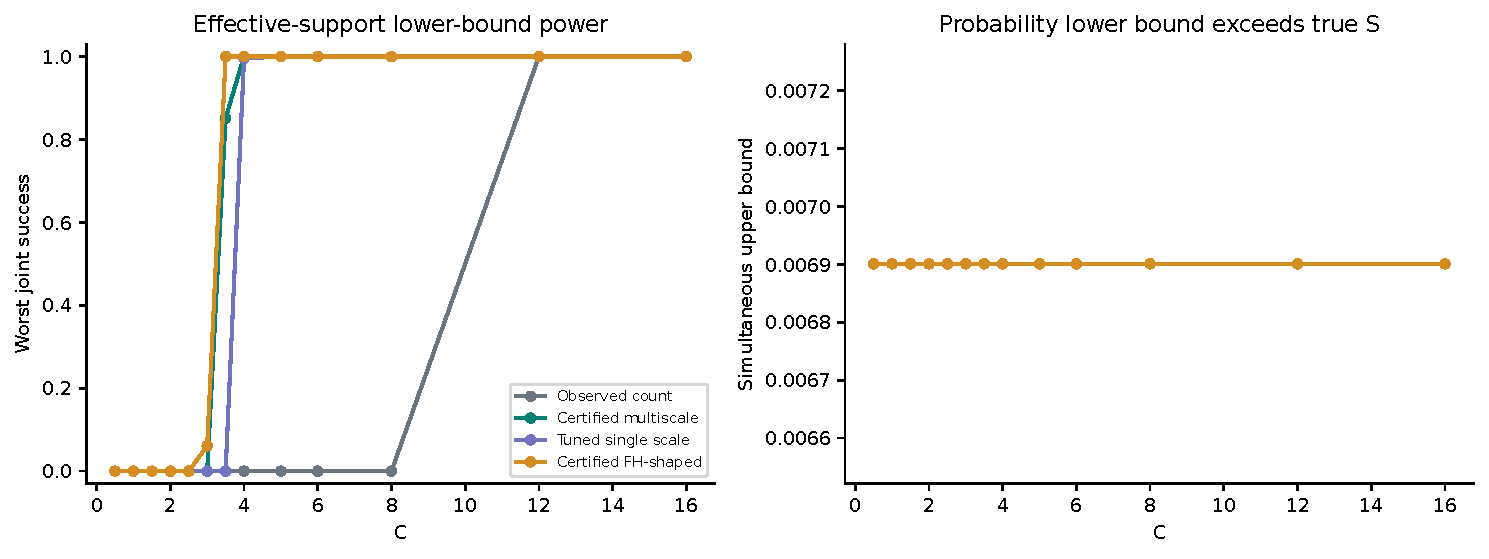
\includegraphics[width=\linewidth]{figures/effective_lower.pdf}\caption{n=10,000, epsilon=0.01. Joint success requires min(effective support,n) <= lower <= S. Exact rational flooring preserves coverage at a cost of less than one category per scale.}\end{figure}
\begin{table}[htbp]\centering\small\caption{Effective-support lower bounds at n=10,000, epsilon=0.01, C=4; all eleven scenarios including Gap are evaluated.}
\resizebox{\linewidth}{!}{
\begin{tabular}{llll}
\toprule
Method & Worst joint success & Worst over-S rate & Mean gain over clipped D \\
\midrule
Observed count & 0.00\% & 0.00\% & 0.0 \\
Certified FH-shaped & 100.00\% & 0.00\% & 2038.6 \\
Certified multiscale & 100.00\% & 0.00\% & 2126.8 \\
Tuned single scale & 99.55\% & 0.00\% & 2122.1 \\
\bottomrule
\end{tabular}
}
\end{table}
\section*{9. Natural groups, held-out groups, and sampling-design repair}
We use NIPS word counts, Enron word counts, MovieLens 1M ratings, Online Retail product rows, BCI tree counts, and the 2007 seine stratum of Inch Lake fish captures [6-10]. Units are documents, users, invoices, spatial quadrats and capture events where available. These published records define finite empirical reference distributions. Their observed support is not asserted to be the support of an external population, and individual records are not automatically independent.

\begin{table}[htbp]\centering\small\caption{Finite empirical reference populations used in the new group-structure experiments.}
\resizebox{\linewidth}{!}{
\begin{tabular}{llll}
\toprule
Dataset & Records & Observed categories & Natural groups \\
\midrule
nips & 1,932,365 & 12,375 & 1,500 \\
enron & 6,412,172 & 28,099 & 39,861 \\
movielens & 1,000,209 & 3,706 & 6,040 \\
retail & 527,725 & 3,791 & 19,773 \\
bci & 21,457 & 225 & 50 \\
fish\_2007\_seine & 1,180 & 8 & 15 \\
\bottomrule
\end{tabular}
}
\end{table}
The UCI text corpora use a publisher-filtered vocabulary, so their rare tails are not an uncensored language distribution. Retail samples are positive-quantity, positive-price product rows, not quantity-expanded independent transactions. BCI is the published 1982 large-tree subset; years are not pooled. Fish records are restricted to one year and one gear. Original licenses, download hashes, filtering rules and sample units are retained in the data provenance manifests.

\begin{figure}[htbp]\centering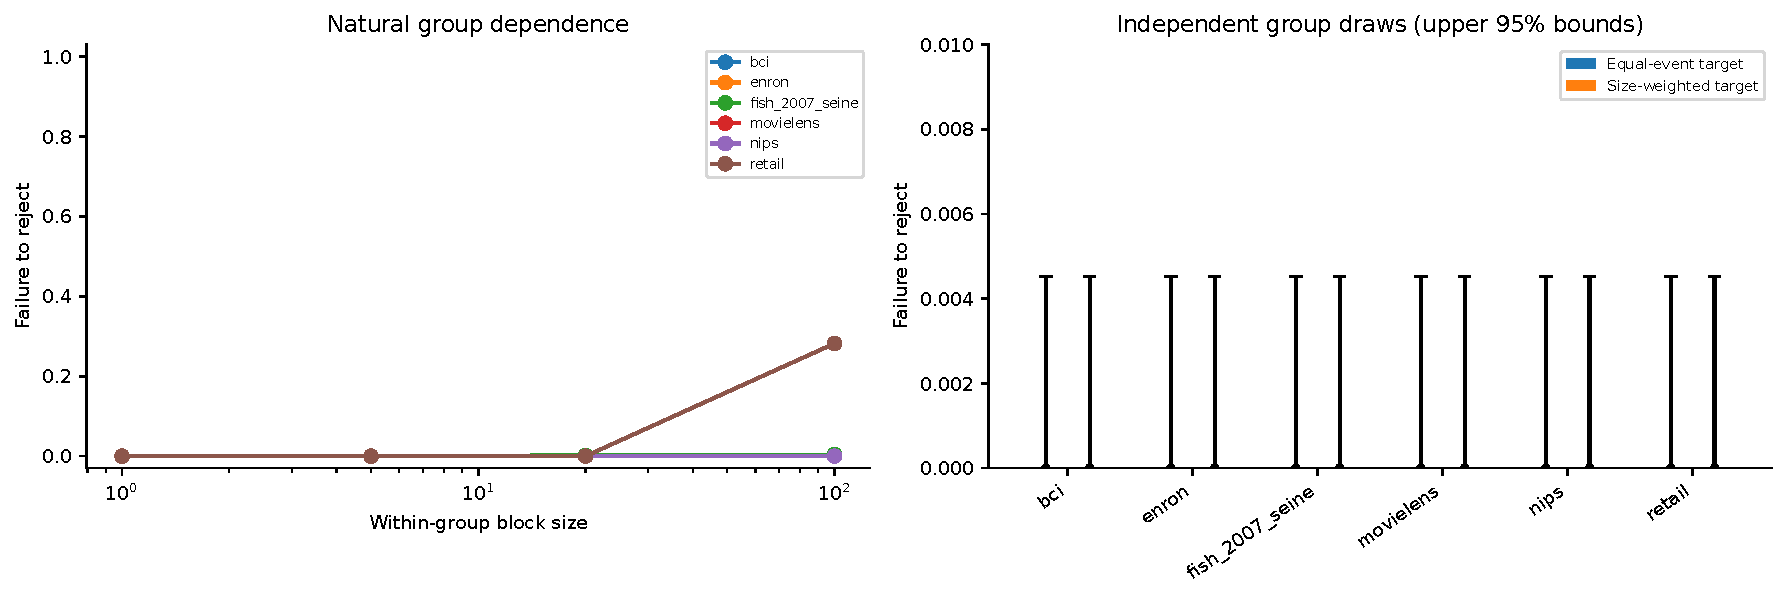
\includegraphics[width=\linewidth]{figures/group_structure.pdf}\caption{Dependent blocks deliberately violate iid. The repaired samplers draw a fresh independent group per label; equal-event weighting changes the target distribution. The right panel has a different vertical scale and shows simultaneous upper confidence limits even at zero observed errors. Fixed-budget non-rejection remains Inconclusive.}\end{figure}
Natural-group stress samples preserve the original marginal record distribution but draw blocks of 5,20,100 observations from the same group. The largest observed multiscale non-rejection rate over these tested No scenarios is 28.20\%. The iid certificate does not apply to those correlated experiments. The fixed-budget output is Inconclusive when evidence is insufficient; interpreting it as a certified Yes would be incorrect.

A repair experiment draws a fresh group independently for every retained label. Size-proportional group selection followed by a uniform record preserves the original record distribution. Uniform group selection defines a distinct event-weighted target, which is reported separately. Three group-disjoint splits per dataset additionally test transfer to new empirical frequency spectra: query n is chosen on training groups, while truth and error are evaluated on independently resampled held-out-group spectra. This is not a claim of independent field-level population truth.

\begin{table}[htbp]\centering\small\caption{Multiscale evaluation on three group-disjoint holdout splits, two training-defined queries and two budgets. A dash means that no cell belongs to that promise stratum.}
\resizebox{\linewidth}{!}{
\begin{tabular}{lllll}
\toprule
Dataset & Cells & Max null error & Max non-rejection & Mean joint lower success \\
\midrule
bci & 12 & 0.00\% & 0.00\% & 100.00\% \\
enron & 12 & 0.00\% & 0.00\% & 100.00\% \\
fish\_2007\_seine & 12 & 0.00\% & 0.00\% & 100.00\% \\
movielens & 12 & 0.00\% & 0.00\% & 100.00\% \\
nips & 12 & 0.00\% & 0.00\% & 100.00\% \\
retail & 12 & -- & 0.00\% & 100.00\% \\
\bottomrule
\end{tabular}
}
\end{table}
\section*{10. Sensitivity, reference branches, and computational cost}
\begin{figure}[htbp]\centering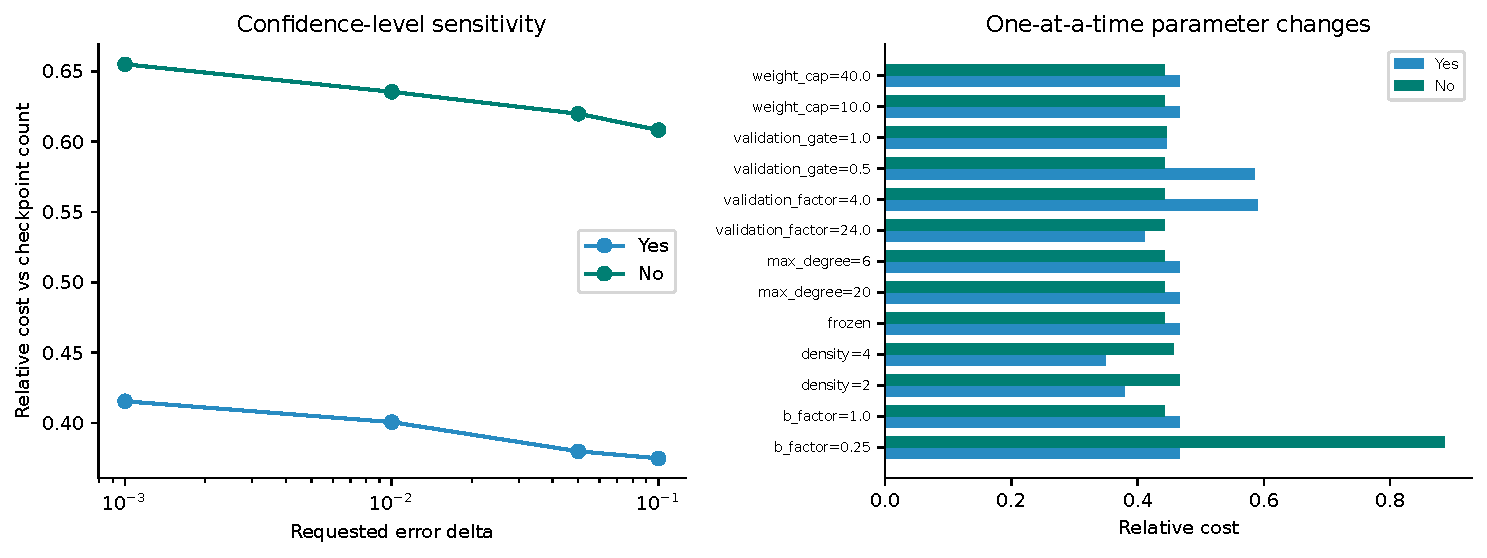
\includegraphics[width=\linewidth]{figures/sensitivity.pdf}\caption{Frozen configurations are not re-selected from these outcomes. Delta=0.001 cells use 20,000 trials; remaining sensitivity cells use 2,000.}\end{figure}
Confidence sensitivity covers delta=0.1,0.05,0.01,0.001; the smallest delta uses 20,000 trials per cell. One-at-a-time changes vary B, degree cap, weight cap, validation allocation, gating and checkpoint density. These outcomes are diagnostic and never reselect the submitted configuration. Failure to establish a small error target by an empirical confidence bound is distinguished from violation of the analytical guarantee.

\begin{table}[htbp]\centering\small\caption{Confidence-level stress: worst rates and simultaneous upper limits over tested multiscale-hybrid cells. An empirical upper limit can exceed the requested risk even when the analytical guarantee applies.}
\resizebox{\linewidth}{!}{
\begin{tabular}{lllll}
\toprule
Target delta & Trials/cell & Max FP & Max FN & Max simultaneous upper \\
\midrule
0.001 & 20000 & 0.00\% & 0.04\% & 0.13\% \\
0.010 & 2000 & 0.00\% & 0.25\% & 1.00\% \\
0.050 & 2000 & 0.00\% & 0.15\% & 0.81\% \\
0.100 & 2000 & 0.00\% & 0.05\% & 0.60\% \\
\bottomrule
\end{tabular}
}
\end{table}
\begin{table}[htbp]\centering\small\caption{Literal finite-scale reference branches, amplified conservatively to at most 5\% error. Costs are prescribed sampling budgets, not simulation runtime.}
\resizebox{\linewidth}{!}{
\begin{tabular}{llll}
\toprule
n & epsilon & Wang total mean & FH fixed samples \\
\midrule
100 & 0.010 & 2,753,714,554,227 & 303,000 \\
100 & 0.100 & 275,371,455,425 & 30,300 \\
1,000 & 0.010 & 19,518,862,402,131 & 3,003,000 \\
1,000 & 0.100 & 1,951,886,240,220 & 300,300 \\
\bottomrule
\end{tabular}
}
\end{table}
For the literal Wang constants, every tested realistic n lies in the observed-count branch. For the explicit FH constant a=1/128, all tested reference epsilon values lie in its small-epsilon branch; Proposition 2.2 with n+1 gives a fixed count tester. Independent majority repetition uses the stated worst-case error bounds, including the 1/10 Markov bound in the FH proof. We simulate the actual Poisson or fixed-multinomial models accordingly. These conservative reference costs are useful provenance checks but not the sole practical baseline; the immediate count baseline is much stronger.

\begin{figure}[htbp]\centering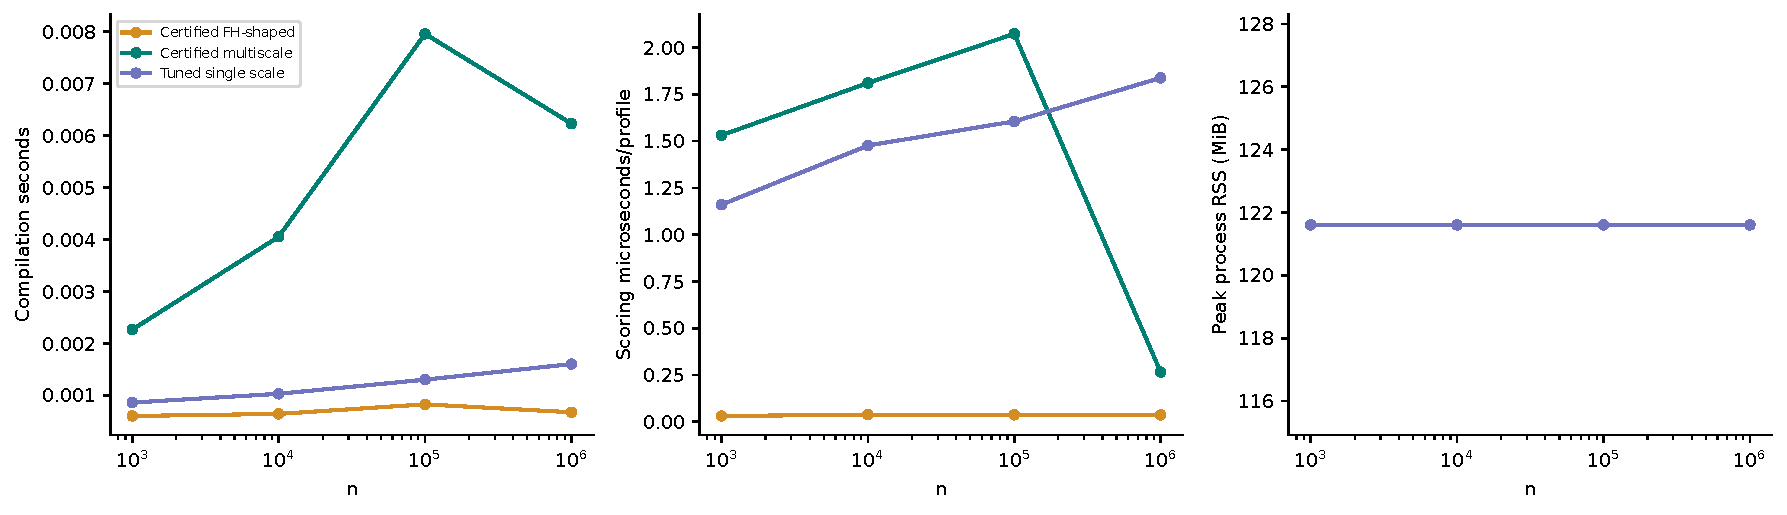
\includegraphics[width=\linewidth]{figures/runtime.pdf}\caption{Compilation is measured separately from grouped simulation and scoring. Peak RSS is the absolute fresh-process peak, including Python and dependencies. Timing should be interpreted on the recorded machine.}\end{figure}
We separate parameter compilation, grouped simulation and decision scoring. Scoring includes integer certification of candidate crossings. Runtime uses fresh processes, one BLAS thread and nine scoring repetitions; peak RSS includes the interpreter and dependencies. Compression makes simulation of enormous known supports computationally feasible, but does not reduce the number of observations that a real sampling procedure must acquire.

\section*{11. Limitations and research claims}
This study establishes a reproducible operating picture for a particular certified construction and finite set of distributions. It does not establish distribution-free acceleration over immediate counting, a minimax lower bound for the hybrid, or a new n/(epsilon log n) guarantee. Development and test shapes belong to overlapping broad distribution families even though parameters and random streams are separated. Adversarial selection explores only a specified family. Actual labelled-stream experiments stop at n=1,000; larger grids use an expected-cost surrogate with an explicit interpretation.

The empirical data do not provide an independent inventory of all species in a lake or all categories in an unseen population. No new field survey was performed. Group resampling addresses a defined empirical target; it does not automatically correct unknown capture probabilities, drift or unseen categories. Native-threshold FH-shaped and Chao1 baselines are heuristic diagnostics, not guaranteed competitors under the full promise model.

A top-tier submission additionally requires an independently assessed novelty claim and venue-specific positioning. The proposed finite-sample composition uses established ingredients, so its theoretical novelty should not be presumed from the size of the experimental package. This manuscript is a complete, evidence-linked research draft; it is not a representation that a venue has accepted it or that experiments alone suffice for acceptance.

\section*{12. Reproducibility}
The artifact contains the frozen design, correctness amendment, selected development configurations, source snapshots, dependency versions, data hashes, exact boundary certificates, raw trial arrays, per-cell CSVs, plotting/analysis code, PDF figures and this manuscript in HTML, PDF and LaTeX. The result audit rechecks original source/data hashes and verifies summary statistics against raw outcomes. Formal and smoke outputs are separate. Historical and superseded experiments are not silently relabelled as new results.

From the project root, create a compatible Python environment, install requirements-lock.txt plus reportlab==4.4.4, and run: OPENBLAS\_NUM\_THREADS=1 OMP\_NUM\_THREADS=1 python -m publication.run --phase all --out results\_reproduction. Original data can be reconstructed with python run\_large\_benchmark.py --phase prepare. Raw and derived source datasets, especially MovieLens, are omitted from the portable package; their download scripts, provenance and hashes are included. Reproduction does not require new tuning on formal outcomes.

\section*{13. Conclusion}
Certified polynomial rejection and independent validation can save observations in complementary regimes. The magnitude of the benefit depends strongly on the count stopping rule, distribution shape, confidence level and sampling design. Reporting exact risk control, practical power, actual acquisition cost and dependence failures separately is essential for interpreting support-size testing experiments.

\section*{References}
[1] Qisheng Wang. Optimal Support Size Testing. Supplied manuscript 2610.18723v1.pdf. \url{https://arxiv.org/abs/2610.18723}


[2] Renato Ferreira Pinto Jr. and Nathaniel Harms. Testing Support Size More Efficiently Than Learning Histograms. TheoretiCS 5, 2026; arXiv:2410.18915v4. \url{https://arxiv.org/abs/2410.18915v4}


[3] Yihong Wu and Pengkun Yang. Chebyshev polynomials, moment matching, and optimal estimation of the unseen. arXiv:1504.01227. \url{https://arxiv.org/abs/1504.01227}


[4] I (Eli) Chien and Olgica Milenkovic. Support Estimation via Regularized and Weighted Chebyshev Approximations. arXiv:1901.07506v2. \url{https://arxiv.org/abs/1901.07506v2}


[5] Steven R. Howard et al. Time-uniform, nonparametric, nonasymptotic confidence sequences. arXiv:1810.08240. \url{https://arxiv.org/abs/1810.08240}


[6] David Newman. Bag of Words. UCI Machine Learning Repository. DOI:10.24432/C5ZG6P. \url{https://archive.ics.uci.edu/dataset/164/bag+of+words}


[7] F. Maxwell Harper and Joseph A. Konstan. The MovieLens Datasets: History and Context. DOI:10.1145/2827872. \url{https://grouplens.org/datasets/movielens/1m/}


[8] Daqing Chen. Online Retail. UCI Machine Learning Repository. DOI:10.24432/C5BW33. \url{https://archive.ics.uci.edu/dataset/352/online+retail}


[9] BCI forest tree counts distributed with vegan; underlying ecological source Condit et al. (2002). \url{https://vegandevs.github.io/vegan/reference/BCI.html}


[10] Derek H. Ogle / FSAdata. InchLake1 fish capture records. \url{https://fishr-core-team.github.io/FSAdata/reference/InchLake1.html}


\end{document}